\documentclass[xcolor = {svgnames,x11names}]{beamer}

\mode<presentation> {
  \usetheme{Malmoe}
  % ou autre ...

  \setbeamercovered{transparent}
  % ou autre chose (il est également possible de supprimer cette ligne)
}


%\usepackage[english]{babel}
% or autre comme par exemple \usepackage[english]{babel}

%\usepackage[latin1]{inputenc}
% or autre

\usepackage{times}
%\usepackage[T1]{fontenc}
% Or autre. Notez que le codage et la fonte doivent être assortis. Si T1
% ne paraît pas très esthétique, essayer d'effacer la ligne contenant fontenc.

\usepackage{color}
\usepackage{tikz}
\usepackage{algorithm}
\usepackage{algorithmic}
\usepackage{hyperref}
\usepackage{multimedia}
\usepackage{listings}

\newcommand\vect[1]{\textbf{#1}}
\newcommand\CS{{\cal C}}
\newcommand\rational{\mathbb{Q}}
\newcommand\real{\mathbb{R}}
\newcommand\Sone{\mathbb{S}^1}
\newcommand\conf{\textbf{q}}
\newcommand\x{\vect{x}}
\newcommand\y{\vect{y}}
\newcommand\z{\vect{z}}
\newcommand\WS{{\cal W}}
\newcommand\robot{{\cal R}}
\newcommand\body{{\cal B}}
\newcommand\obst{{\cal O}}
\newcommand\CSobst{\CS_{obst}}
\newcommand\CSfree{\CS_{free}}
\newcommand\sturm{\textbf{sturm}}
\newcommand\var{\textbf{n}_{chsgn}}
\newcommand\nor{\textbf{nr}}
\newcommand\signe{\textbf{signe}}
\newcommand\Kappa{{\cal K}}
\newcommand\calP{{\cal P}}
\newcommand\moment{\vect{M}}
\newcommand\resultante{\vect{R}}
\newcommand\f{\vect{f}}
\newcommand\vel{\vect{v}}
\newcommand\gravity{\vect{g}}
\newcommand\trans{\vect{t}}
\newcommand\rotation{R}
\newcommand\utheta{u_{\theta}}

\definecolor{grey}{rgb}{0.5,0.5,0.5}


\title[The stack of tasks] {The stack of tasks - Part 2}

\subtitle{}

\author[]
{Florent Lamiraux, \textcolor{red}{Olivier Stasse} and Nicolas Mansard}

\institute[CNRS-LAAS] % (facultatif mais généralement nécessaire)
{
  CNRS-LAAS, Toulouse, France
}
\date[] % (facultatif, peut être une abréviation du nom de la conférence)
{}

\AtBeginSection[]{
  \begin{frame}<beamer>
    \frametitle{Outline}
  \tableofcontents[currentsection]
  \end{frame} 
}

\AtBeginSubsection[]{
  \begin{frame}<beamer>
    \frametitle{Outline}
  \tableofcontents[currentsection, currentsubsection]
  \end{frame} 
}

\begin{document}

\lstset{
breakatwhitespace=true,
%language=C++,
%columns=fullflexible,
%keepspaces=true,
breaklines=true
tabsize=3, 
%showstringspaces=false,
%extendedchars=true
}

\begin{frame}
  \titlepage
\end{frame}

%\input{intro}
\begin{frame}{The stack of tasks}
  \tableofcontents[currentsection,currentsubsection]
  % Vous pouvez, si vous le souhaiter ajouter l'option [pausesections]
\end{frame}
\section{Introduction}
%
%  Introduction
%


\begin{frame} {Introduction}
  \begin{block}{Part 1 - A Quick Reminder}
    \begin{itemize}
      \item Theoritical Foundations
      \item Fundamental repositories and their role
      \item Installation procedure
    \end{itemize}
  \end{block}
  \begin{block}<2>{Part 2 - A Quick Appetizer}
    \begin{itemize}
      \item Quick start
      \item Software structure
    \end{itemize}
  \end{block}
\end{frame}

\section{Quick start}

\begin{frame}[fragile]{An example with HRP-2}
  \begin{block}{Assumptions}
    \begin{itemize}
      \item OpenHRP 3.0.7 is installed
      \item The Stack of Tasks has been installed thanks to Florent slides with
        \textbf{install\_sot.sh} in the directory:
        \begin{lstlisting}[language=bash,basicstyle=\small,frame=single,showlines=false]    
          /home/user/devel/ros_unstable
        \end{lstlisting}
      \item Your /opt/grx3.0/HRP2LAAS/bin/config.sh is well setup.
    \end{itemize}
  \end{block}
  \begin{block}{The golden commands}
  \begin{lstlisting}[language=bash,basicstyle=\tiny,backgroundcolor=\color{AliceBlue}, frame=single,showlines=false]
    $>roscore
    #Launching HRP2 simulation with OpenHPR
    $>roslaunch hrp2_bringup openhrp_bridge.launch robot_machine_profile:=sim
    $>rosservice call /start_dynamic_graph 
    $>rosrun dynamic_graph_bridge run_command
  \end{lstlisting}
  \end{block}
\end{frame}

\begin{frame}[fragile]{An example}
\begin{block}{Import the graph python module}
  \begin{lstlisting}[language=Python,basicstyle=\small,backgroundcolor=\color{AliceBlue}, frame=single,showlines=false]
[INFO] [WallTime: 1370854858.786392] waiting for service...
Interacting with remote server.
>>> from dynamic_graph.sot.pattern_generator.walking import *
With meta selector
  \end{lstlisting}
\end{block}
\end{frame}


\begin{frame}[fragile]{An example}
\begin{block}{Create the graph}
  \begin{lstlisting}[language=Python,basicstyle=\small,backgroundcolor=\color{AliceBlue}, frame=single,showlines=false]
>>> CreateEverythingForPG(robot,solver)
At this stage
('modelDir: ', '~/devel/ros-unstable/install/share/hrp2-14')
('modelName:', 'HRP2JRLmainsmall.wrl')
('specificitiesPath:', 'HRP2SpecificitiesSmall.xml')
('jointRankPath:', 'HRP2LinkJointRankSmall.xml')
After Task for Right and Left Feet
  \end{lstlisting}
\end{block}
\end{frame}


\begin{frame}[fragile]{An example}
  \begin{block}{Switch to the new graph}       
    \begin{lstlisting}[language=Python,basicstyle=\small,backgroundcolor=\color{AliceBlue}, frame=single,showlines=false]
>>> walkFewSteps(robot)
>>> 
    \end{lstlisting}
  \end{block}
\end{frame}

\section{Software Structure}

\begin{frame}{Software structure - Conceptual view}
  \begin{figure}
    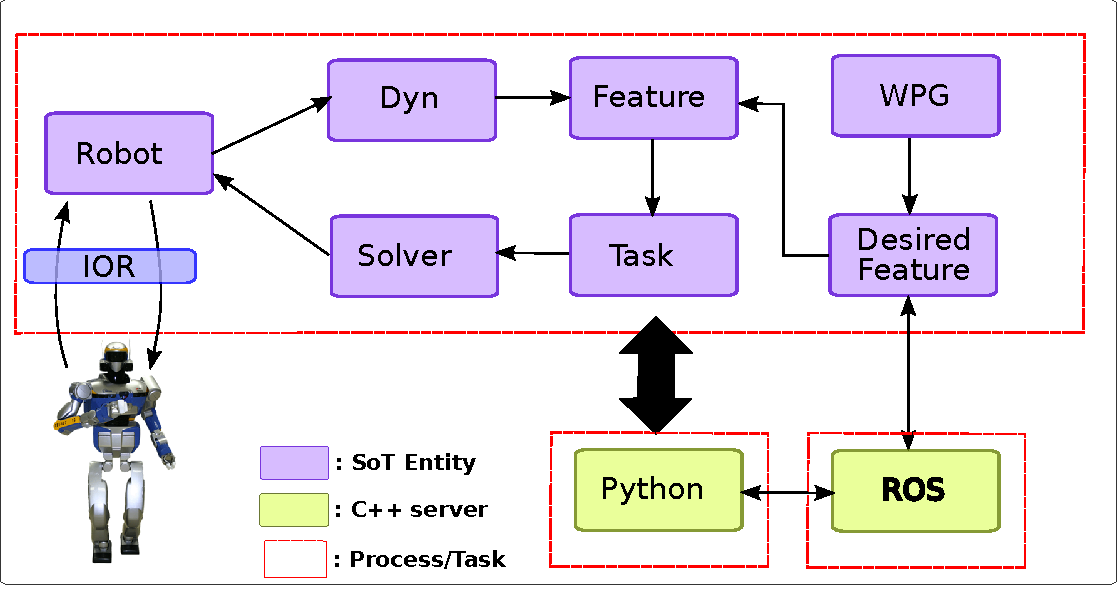
\includegraphics[width=\linewidth]{./figures/Concept-Fig}
  \end{figure}
\end{frame}

\begin{frame}{Software structure - Link with Model}
  \begin{figure}
    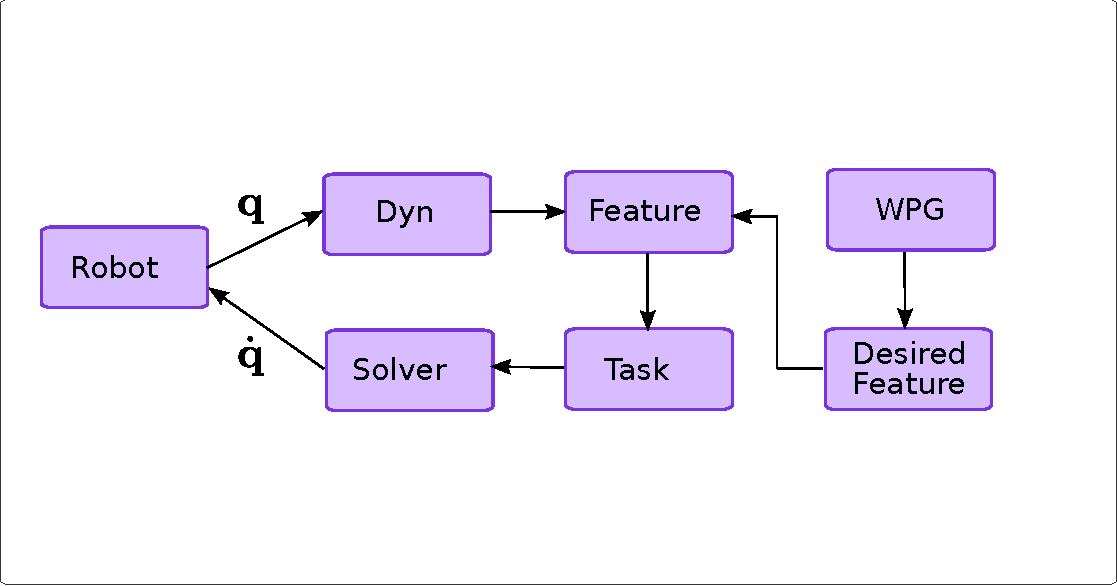
\includegraphics[width=\linewidth]{./figures/Concept-Theory-Fig-Finalv2M5}
  \end{figure}
\end{frame}

%  $$ T ({\bf q}, t) = \left(\begin{array}{cc} {\bf t} (M^{* -1}(t) M ({\bf q})) \\ u_{\theta} (R^{* -1}(t) R ({\bf q})) \end{array}\right) $$
    
% $ J=  \frac{\partial T}{\partial {\bf q}}$
 
% $\dot{T} = - \lambda T

% $\dot{T} = - \lambda T - \frac{\partial T}{\partial t} $

% $\dot{{\bf q}} \triangleq& -J ^{+} (\lambda T + \frac{\partial T}{\partial t} $

\begin{frame}{Software structure - Link with Model}
  \begin{figure}
    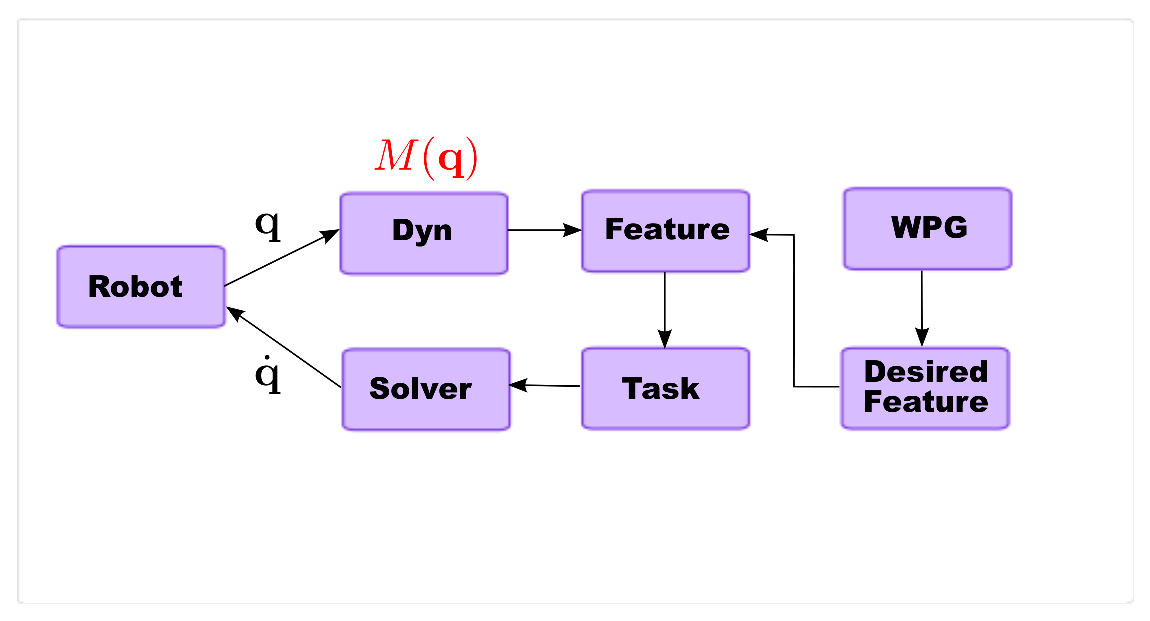
\includegraphics[width=\linewidth]{./figures/Concept-Theory-Fig-Finalv2M4}
  \end{figure}
\end{frame}

\begin{frame}{Software structure - Link with Model}
  \begin{figure}
    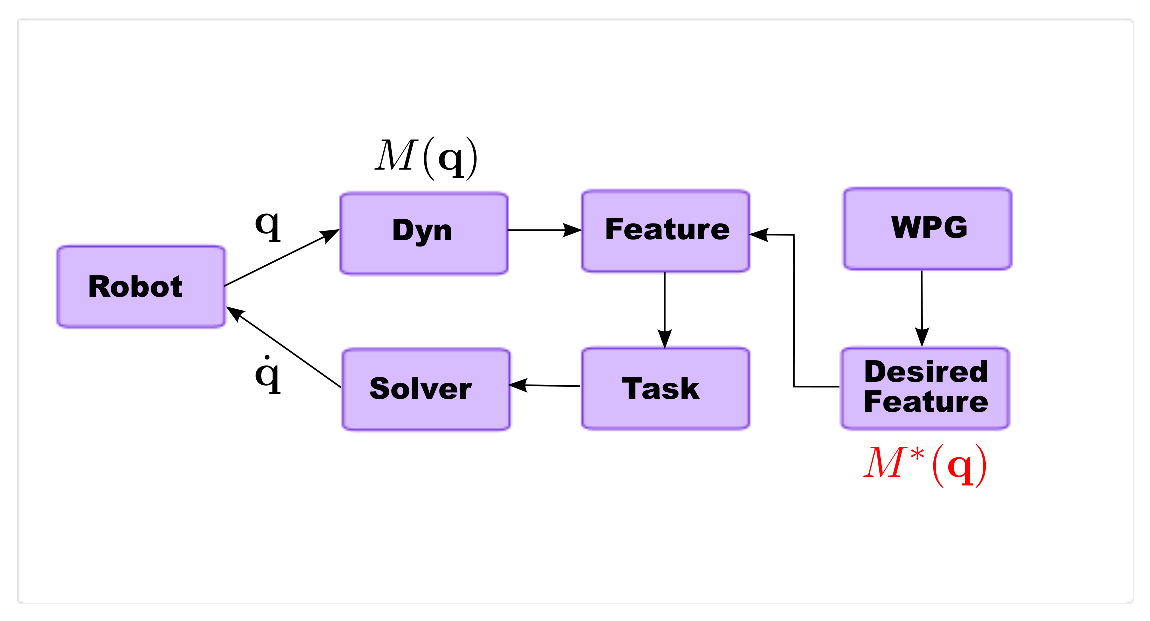
\includegraphics[width=\linewidth]{./figures/Concept-Theory-Fig-Finalv2M3}
  \end{figure}
\end{frame}

\begin{frame}{Software structure - Link with Model}
  \begin{figure}
    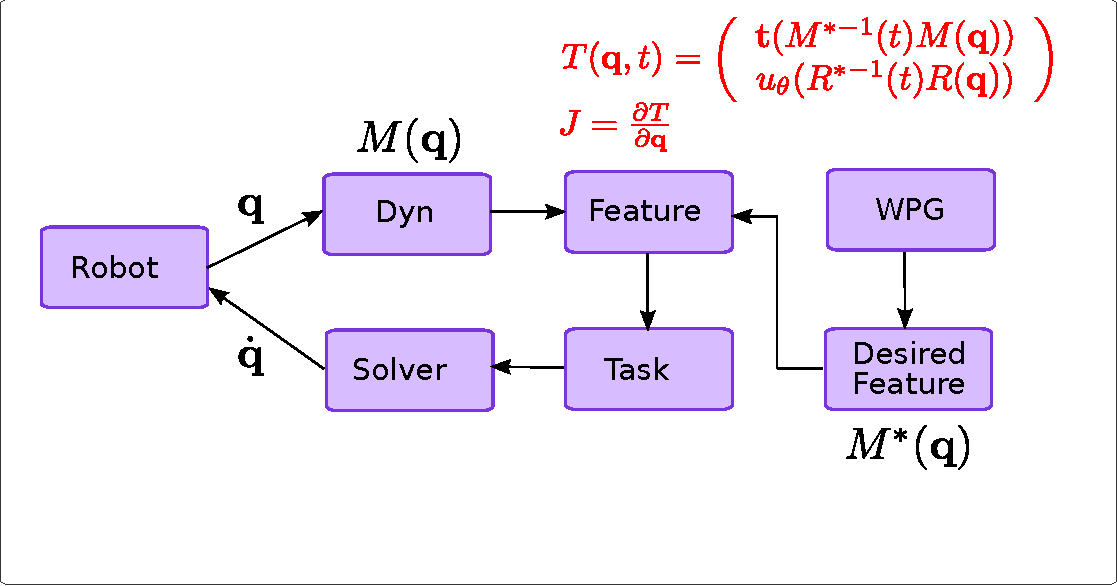
\includegraphics[width=\linewidth]{./figures/Concept-Theory-Fig-Finalv2M2}
  \end{figure}
\end{frame}

\begin{frame}{Software structure - Link with Model}
  \begin{figure}
    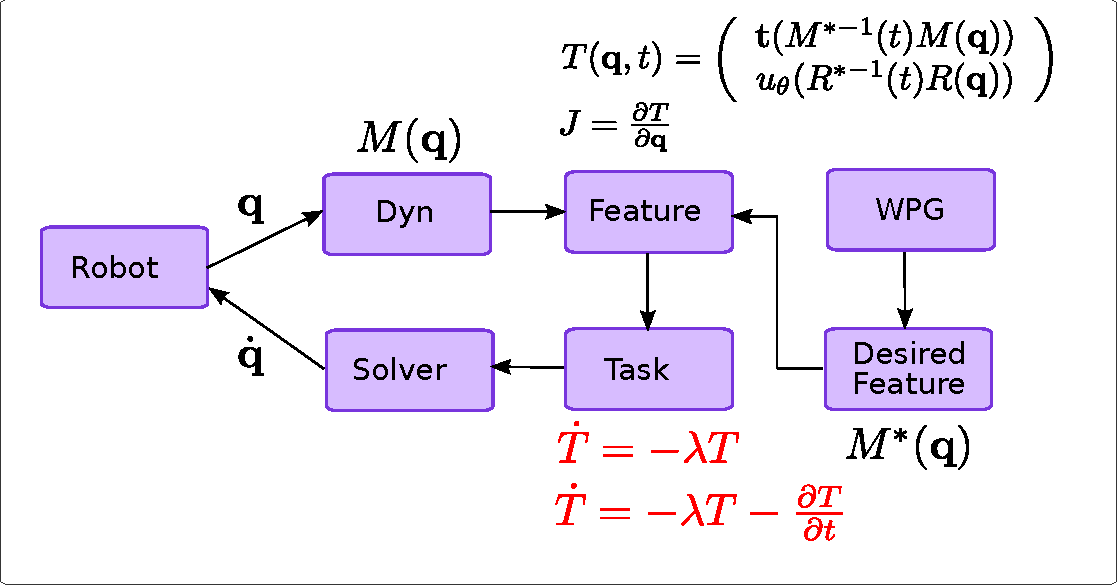
\includegraphics[width=\linewidth]{./figures/Concept-Theory-Fig-Finalv2M1}
  \end{figure}
\end{frame}

\begin{frame}{Software structure - Link with Model}
  \begin{figure}
    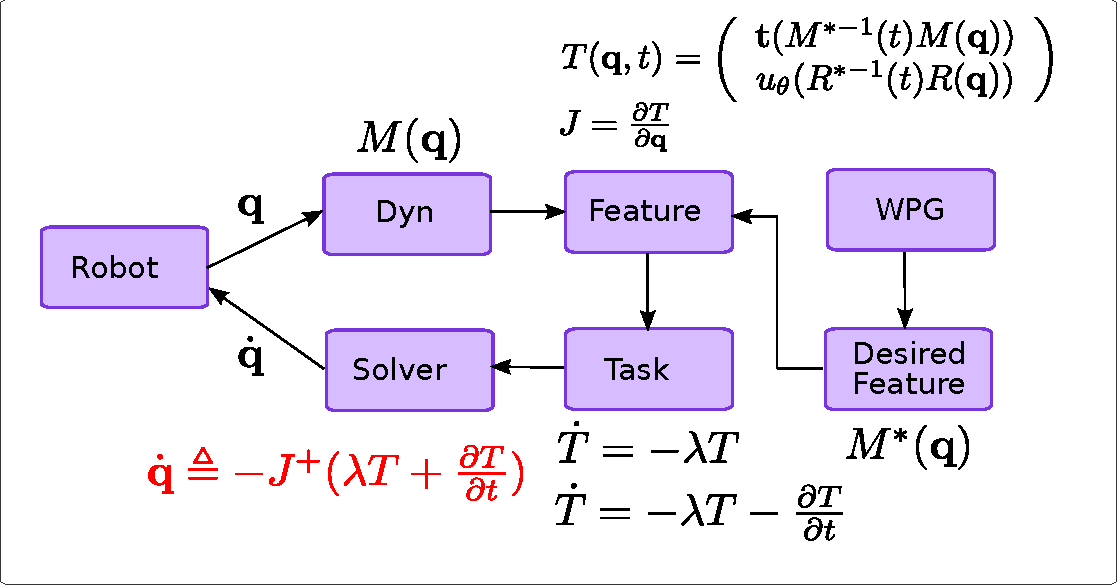
\includegraphics[width=\linewidth]{./figures/Concept-Theory-Fig-Finalv2}
  \end{figure}
\end{frame}

\begin{frame}{Software structure - Repositories}
  \begin{figure}
    \includegraphics[width=\linewidth]{./figures/Concept-Software-Fig}
  \end{figure}
\end{frame}


\end{document}
